\section{Результаты}
\begin{figure}[H]\label{InfSet}
\centering
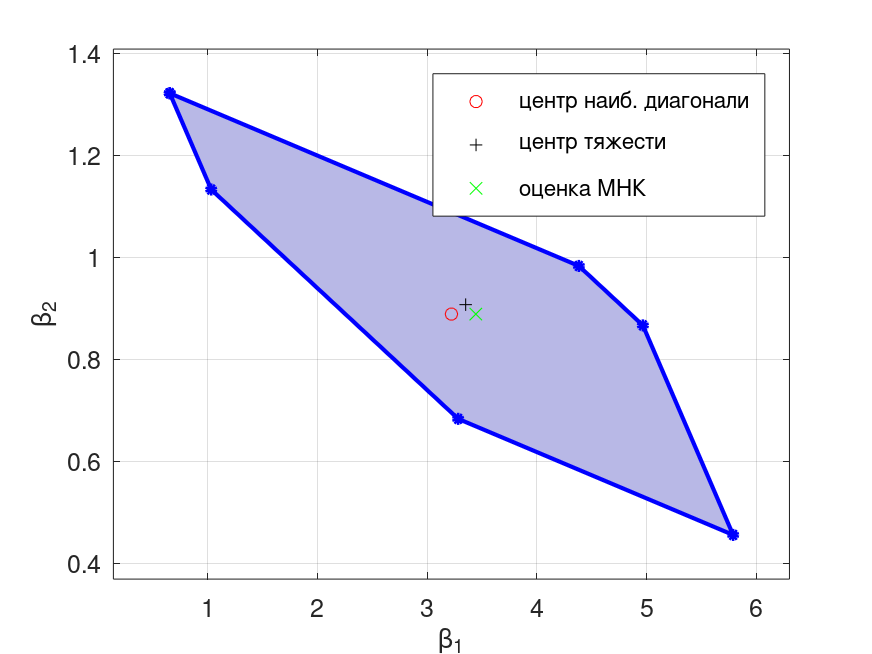
\includegraphics[width=1\textwidth]{Graphics/InformSet.png}
\caption{Информационное множество и точечные оценки задачи \eqref{Task}} 
\end{figure}

Положения оценок:
\begin{equation}
\hat{\beta}_{\mathrm{maxdiag}}=[3.2222, 0.8889], \quad \hat{\beta}_{\mathrm{gravity}} = [3.3519,   0.9074], \quad
\hat{\beta}_{\mathrm{lsm}} = [3.4444,   0.8889]
\end{equation}

\begin{figure}[H]\label{Corridor}
\centering
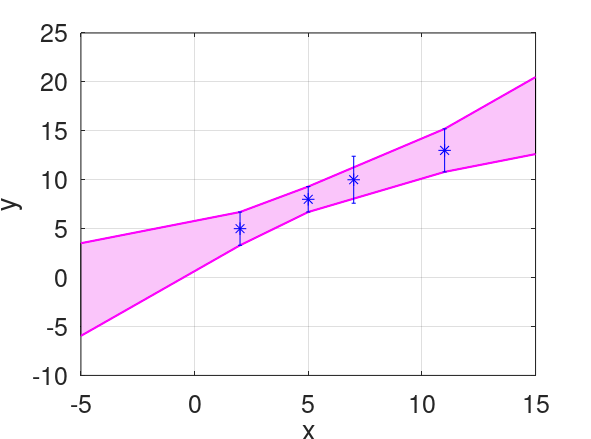
\includegraphics[width=0.9\textwidth]{Graphics/Corridor.png}
\caption{Коридор совместных решений задачи \eqref{Task}} 
\end{figure}
Множество граничных измерений
\begin{equation}
    X_{\mathrm{boundary}}=\{2,5,11\}
\end{equation}
В качестве точек для предсказаний был выбран вектор $x=(-3, 1, 4, 9, 14)^{\mathrm{T}}$
\begin{figure}[H]\label{Predictions}
\centering
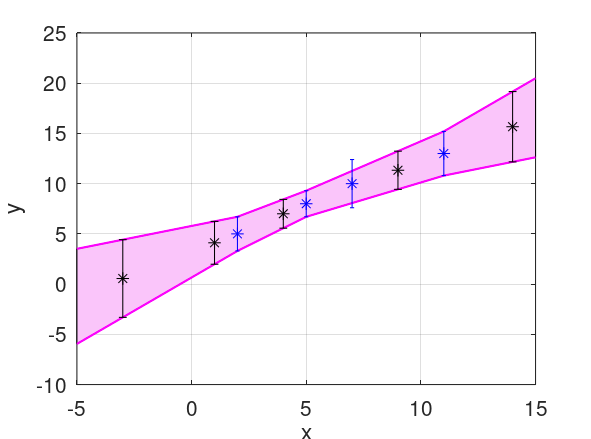
\includegraphics[width=0.9\textwidth]{Graphics/Predictions.png}
\caption{Значения предсказаний задачи \eqref{Task}} 
\end{figure}